\begin{figure}[htbp]
\centering
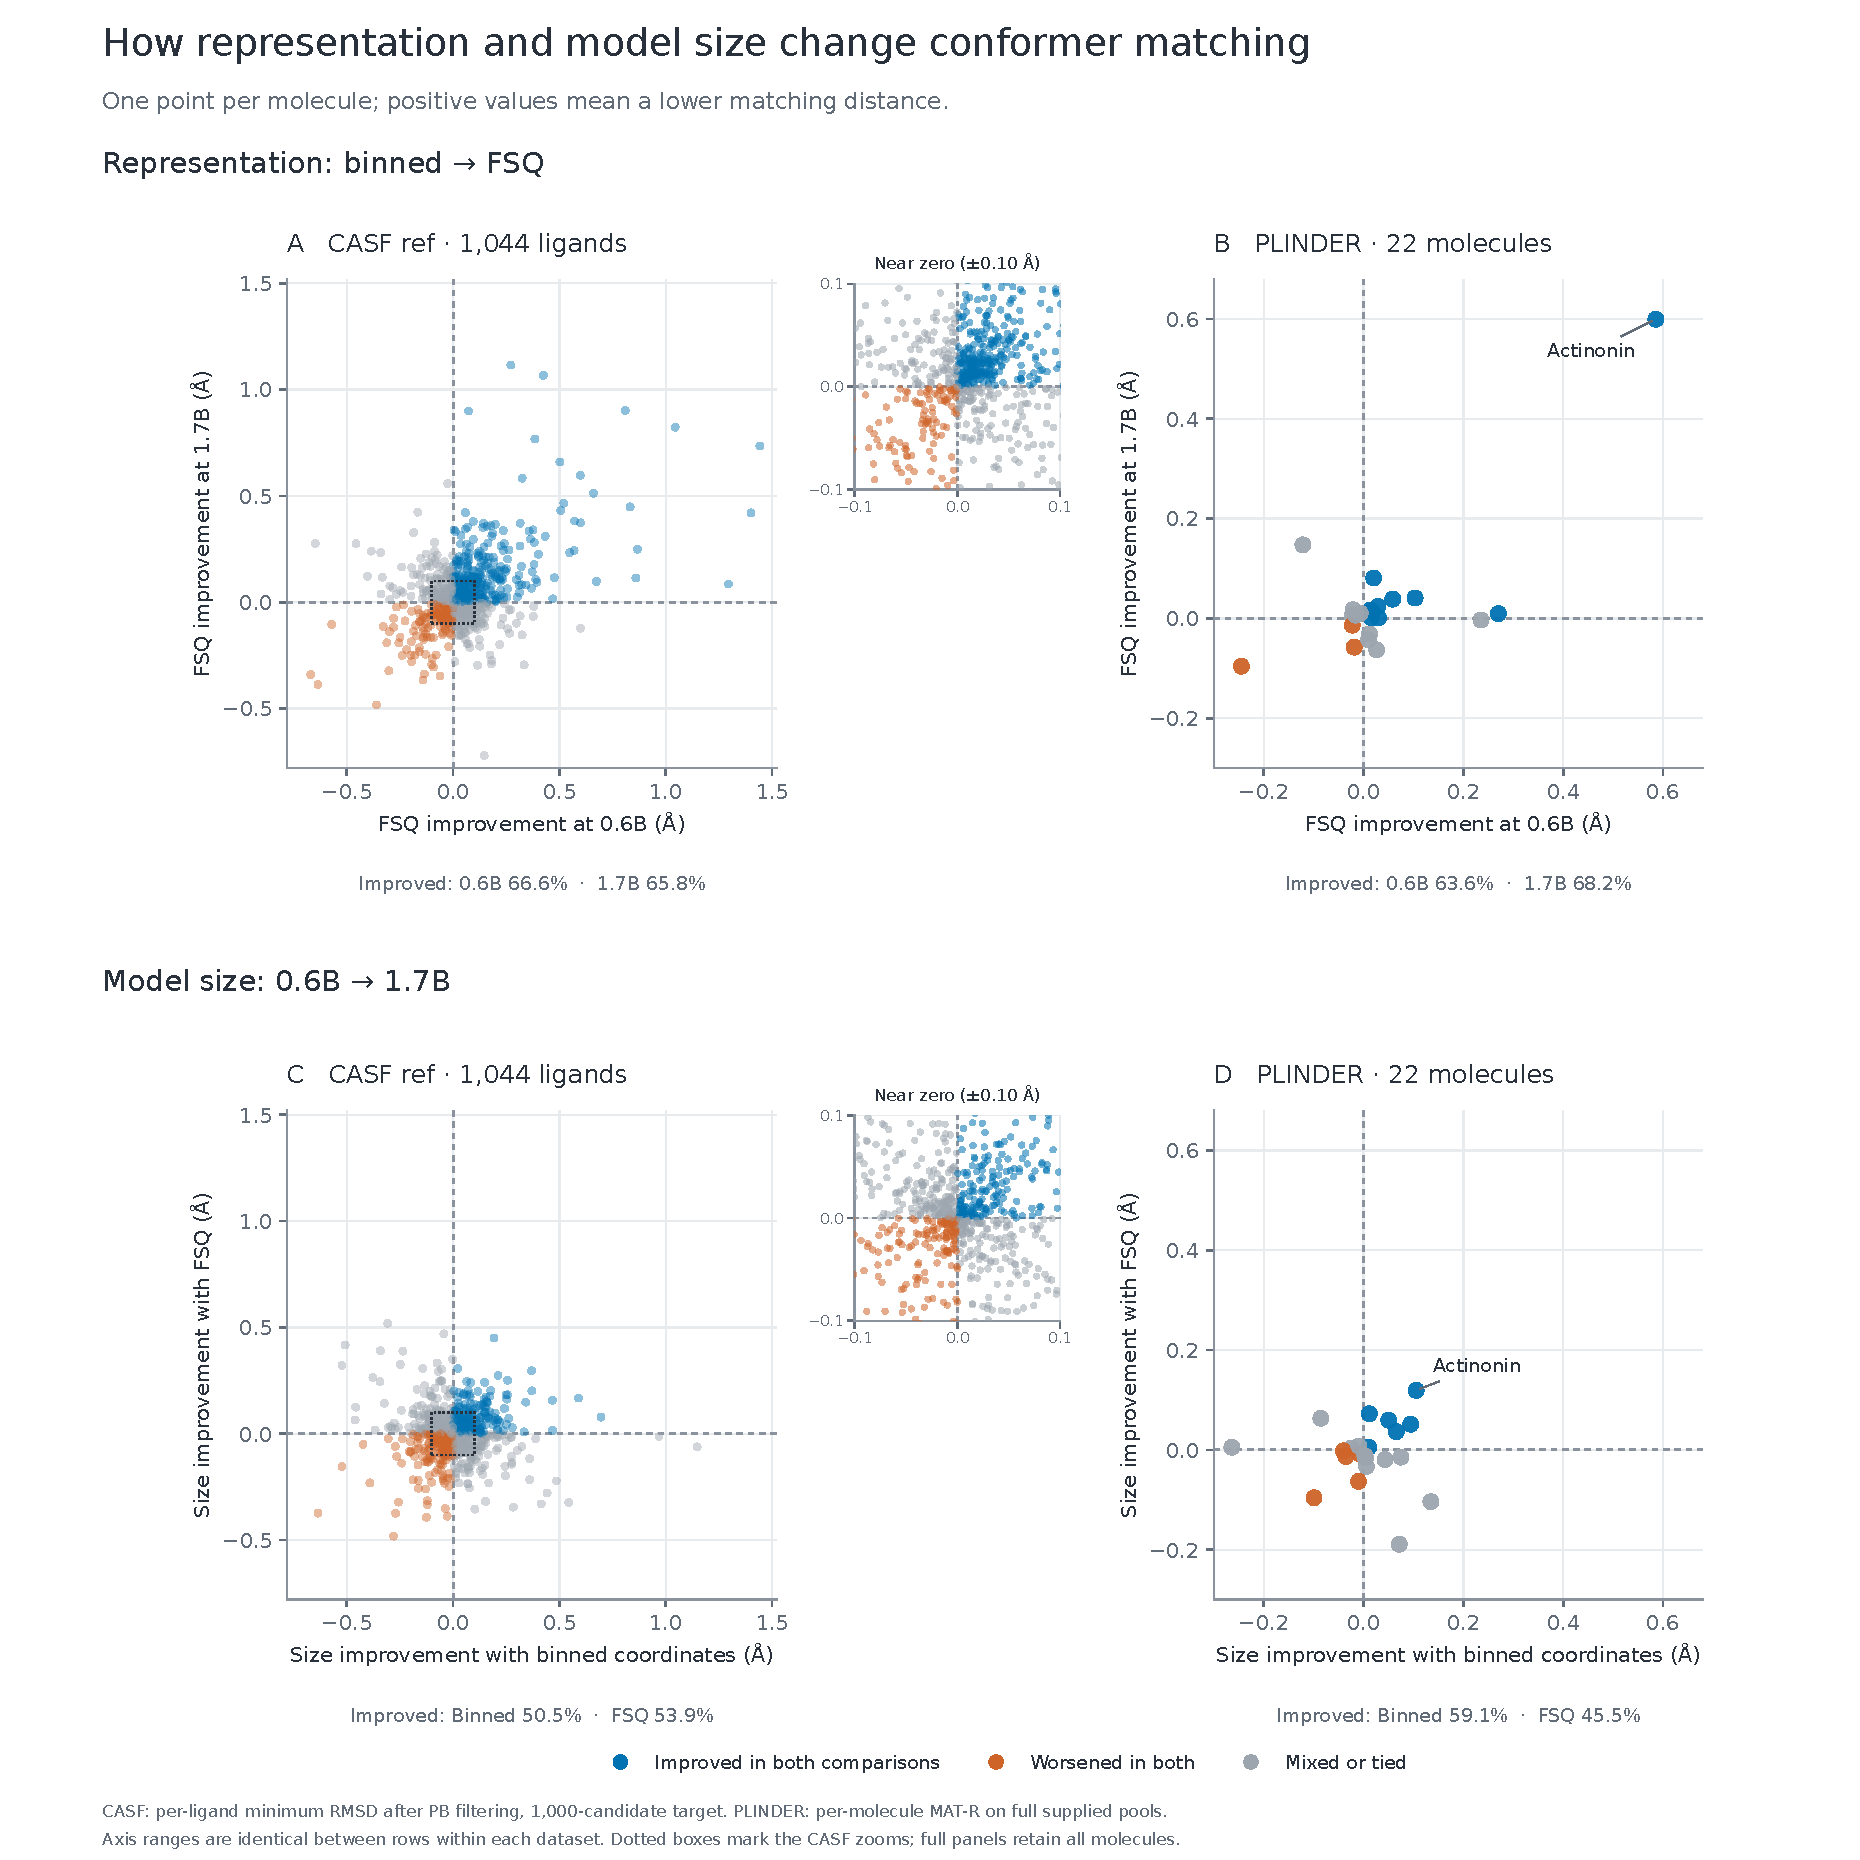
\includegraphics[width=\linewidth,height=0.72\textheight,keepaspectratio]{figures/figure-qwen-molecule-effects.pdf}
\caption{Molecule-level changes in matching distance on CASF ref (A, C) and PLINDER (B, D). Each point represents one ligand or molecule. In A--B, the coordinates are the reductions in distance from binned coordinates to FSQ at 0.6B and 1.7B. In C--D, they are the reductions from 0.6B to 1.7B with binned coordinates and FSQ. Positive values indicate closer matching. Blue denotes improvement in both comparisons, orange worsening in both, and grey mixed or tied outcomes. Percentages below each panel give the fraction improved along each axis. CASF uses per-ligand minimum RMSD; PLINDER uses per-molecule MAT-R. Axis ranges are identical between rows within each dataset. Insets enlarge the dotted CASF regions to $\pm0.10$ \AA{}; full panels retain all molecules. Actinonin is labeled in both PLINDER panels.}
\label{fig:qwen-molecule-effects}
\end{figure}
